% Ceci est un commentaire
% En−tete de tout document LaTeX. Sp´ecifie le type de document ´ecrit
\documentclass[9pt,a4paper]{article}
\usepackage[french]{babel}
\usepackage{epsfig}
\usepackage{graphicx}
\usepackage{tikz}
\usepackage{amssymb} % ensemble des réels, etc
\usepackage{amsmath, amsthm}
\usepackage{fancyhdr}
\usepackage{enumitem}
\usepackage{float}


\usepackage[linesnumbered, ruled, vlined]{algorithm2e}
\renewcommand{\algorithmcfname}{Algorithme}
\SetKwInput{KwData}{Données}
\SetKwInput{KwRes}{Résultat}
\SetKwProg{Fonction}{Fonction}{}{FinFonction}
\SetKwIF{Si}{SinonSi}{Sinon}{Si}{alors}{SinonSi}{Sinon}{FinSi}
\SetKwFor{Pour}{Pour}{faire}{FinPour}
\SetKwFor{Tq}{Tant que}{faire}{FinTantque}
\SetKw{Renvoyer}{Renvoyer}
\usepackage{algpseudocode}

\usepackage{fancyvrb}

\usepackage{biblatex}

%\usepackage{hyperref}

\usepackage[acronym]{glossaries-extra}
\setabbreviationstyle[acronym]{long-short}
\newacronym{rk4}{RK4}{Runge-Kutta d'ordre 4}
\newacronym{edo}{EDO}{Equations Différentielles Ordinaires}
\makeglossaries

\usepackage{tcolorbox}

\usepackage{xcolor}

\usepackage[a4paper,top=2cm,bottom=2cm,left=3cm,right=3cm,marginparwidth=1.75cm]{geometry}

\newtheorem{prop}{Proposition}
\newtheorem{rem}{Remarque}

\title{Rapport Projet\\
Oscillations d'un pendule}
\author{LIMAM Mohamed Selim\\LEFORT Kelvin}


\begin{document}
\maketitle
\newpage
\cfoot{MACS 1 - Sup Galilée - Institut Galilée - Université Sorbonne Paris Nord}
\rfoot{\thepage}
\pagestyle{fancy}
\tableofcontents % ´ecrit la table des mati`eres
\newpage


On utilisera durant tout le projet la méthode de \gls{rk4} car elle est connue pour être une méthode très précise et largement utilisée pour résoudre numériquement des \gls{edo}. On n’étudiera pas les méthodes (stabilité, consistance, ordre, ...) et on ne comparera pas les différentes méthodes (\gls{rk4}, Euler explicite, Euler implicite, Crank-Nicholson, …) entre elles. Cela a été fait durant les TP d’\gls{edo}. On s'arrêtera aux simulations.

\section{Méthode de RK4}
Soient $f : \mathbb{R} \times \mathbb{R}^d \longrightarrow \mathbb{R}^d$ et $y^0 \in \mathbb{R}^d$. Soit $T \in \mathbb{R}_+$. \\
La méthode de \gls{rk4} est une méthode d'approximation numérique d'une \gls{edo} de la forme :
$$
\left\{
  \begin{array}{lcl}
    y'(t) = f(t, y(t)), & t \in I := [0, T] \\
    y(0) = y^0 \\
  \end{array}
\right.
$$
où $f$ et $y^0$ sont les données du problème de Cauchy.
\subsection{Construction de la méthode de RK4}
Soit $N \in \mathbb{N}^*$ fixé. \\
Commençons par discrétiser l'intervalle $I$ en $N$ intervalles de même longueur $h := \frac{T}{N}$. Pour cela, posons $t_n = nh$ et $I_n = [t_n, t_{n + 1}]$ pour $n \in [\![0, N - 1]\!]$ (il y a donc $(N+1)$ points $t_n$). L'objectif est de construire une suite de valeurs $y_0, ..., y_N$ approchant les valeurs $y(t_0), ..., y(t_N)$. Remarquons que puisque $y(0) = y^0$, alors on prend $y_0 = y^0$. \\
Voici la méthode de \gls{rk4} pour construire une telle suite : \\
\begin{tcolorbox}[colback=green!5!white, colframe=green!50!black, title = Méthode de \gls{rk4}]
Soient $(k_{n, 1})_{n \in [\![0, N - 1]\!]}$, $(k_{n, 2})_{n \in [\![0, N - 1]\!]}$, $(k_{n, 3})_{n \in [\![0, N - 1]\!]}$ et $(k_{n, 4})_{n \in [\![0, N - 1]\!]}$ des suites finies à valeurs dans $\mathbb{R}^d$. Alors $(k_{n, 1})_{n \in [\![0, N - 1]\!]}$, $(k_{n, 2})_{n \in [\![0, N - 1]\!]}$, $(k_{n, 3})_{n \in [\![0, N - 1]\!]}$, $(k_{n, 4})_{n \in [\![0, N - 1]\!]}$ et $(y_n)_{n \in [\![0, N]\!]}$ vérifient : \\
$$
\left\{
  \begin{array}{lcl}
    k_{n, 1} = f(t_n, y_n) \\
    k_{n, 2} = f(t_n + \frac{h}{2}, y_n + \frac{h}{2}k_{n, 1}) \\
    k_{n, 3} = f(t_n + \frac{h}{2}, y_n + \frac{h}{2}k_{n, 2}) \\
    k_{n, 4} = f(t_n + h, y_n + hk_{n, 3}) \\
    y_{n + 1} = y_n + \frac{h}{6}(k_{n, 1} + 2k_{n, 2} + 2k_{n, 3} + k_{n, 4}) \\
  \end{array}
\right.
$$
avec $n \in [\![0, N - 1]\!]$.
\end{tcolorbox}
\subsection{Implémentation de la méthode de RK4}
Remarquons que la construction de la suite $(y_n)_{n \in [\![0, N]\!]}$ par la méthode de \gls{rk4} se fait de manière récurrente à un pas (pour déterminer $y_{n + 1}$, on a juste besoin de connaître $y_n$) et de manière explicite (on n'a pas besoin de résoudre d'équations pour déterminer $y_{n + 1}$ à partir de $y_n$). \\
Vous trouverez ci-dessous un pseudo-code qui explique comment construire la suite algorithmiquement :
\begin{algorithm}[H]
    \caption{Méthode de \gls{rk4}}
    \SetAlgoLined
    \DontPrintSemicolon
    \KwData{ \\
        $f : \mathbb{R} \times \mathbb{R}^d \longrightarrow \mathbb{R}^d$ \\
        $y^0 \in \mathbb{R}^d$ \\
        $T \in \mathbb{R}_+$ \\
        $N \in \mathbb{N}^*$ \\
    }
    \KwRes{
        $(y_0, ..., y_N) \in (\mathbb{R}^d)^{N + 1}$
    }
    \Fonction{$(y_0, ..., y_N) \gets$ {\color{red}runge\_kutta\_4} $(f, y^0, T, N)$}{
        $h \gets \frac{T}{N}$ \\
        $y_0 \gets y^0$ \\
        $t \gets 0$ \\
        \Pour{$n \gets 0$ à $(N - 1)$}{
            $k_1 \gets f(t, y_n)$ \\
            $k_2 \gets f(t + \frac{h}{2}, y_n + \frac{h}{2}k_1)$ \\
            $k_3 \gets f(t + \frac{h}{2}, y_n + \frac{h}{2}k_2)$ \\
            $k_4 \gets f(t + h, y_n + hk_3)$ \\
            $y_{n + 1} \gets y_n + \frac{h}{6}(k_1 + 2k_2 + 2k_3 + k_4)$ \\
            $t \gets t + h$ \\
        }
        \Renvoyer{$(y_0, ..., y_N)$}
    }
\end{algorithm}
Voyons à présent comment écrire cet algorithme en langage C. \\
La première question qui se pose est comment représenter un vecteur de $\mathbb{R}^d$. Quoi de mieux qu'une structure pour le faire : \\
\begin{Verbatim}[numbers=left, frame=single]
#define TAILLE_MAX 10
typedef struct Vecteur_s
{
    int d; // taille du vecteur, en supposant que d <= TAILLE_MAX
    double x[TAILLE_MAX]; //coeficients du vecteur
}Vecteur_t;
\end{Verbatim}
Il faut ensuite écrire les opérations $+$ entre deux vecteurs et $.$ entre un scalaire et un vecteur. \\
Pour cela, on créera deux fonctions, somme\_vecteur et produit\_vecteur : \\
\begin{Verbatim}[numbers=left, frame=single]
Vecteur_t somme_vecteur(Vecteur_t u, Vecteur_t v)
{
    Vecteur_t w;

    w.d = u.d;
    for (int i = 0 ; i < w.d ; i++)
    {
        w.x[i] = u.x[i] + v.x[i];
    }

    return w;
}

Vecteur_t produit_vecteur(double lambda, Vecteur_t u)
{
    Vecteur_t v;

    v.d = u.d;
    for (int i = 0 ; i < v.d ; i++)
    {
        v.x[i] = lambda*u.x[i];
    }

    return v;
}
\end{Verbatim}
On regroupera alors la structure Vecteur\_t et les deux fonctions dans les fichiers vecteur.h et vecteur.c.\\
On se demande désormais comment représenter la fonction $f$ en C et comment la donner en paramètre par la suite à la fonction runge\_kutta\_4 (on écrira cette fonction après).\\
Pour la représentation de $f$, rien de plus trivial qu'une fonction :\\
\begin{Verbatim}[numbers=left, frame=single]
Vecteur_t f(double t, Vecteur_t y)
{
    Vecteur_t z;

    // contenu de la fonction f selon le problème en question

    return z;
}
\end{Verbatim}
On mettra cette fonction et sa déclaration dans les fichiers f.h et f.c.\\
Pour pouvoir donner la fonction f en paramètre, nous utiliserons les pointeurs de fonctions. Nous y reviendrons lors de l'écriture de la fonction runge\_kutta\_4.\\
Enfin, pour écrire l'algorithme runge\_kutta\_4 en C, nous écrirons une fonction et pour stocker le résultat $(y_0, ..., y_N)$, on allouera dynamiquement un tableau de (N+1) cases, chacune pouvant stocker une structure Vecteur\_t :\\
\begin{Verbatim}[numbers=left, frame=single]
Vecteur_t* runge_kutta_4(Vecteur_t (*f)(double t, Vecteur_t y), Vecteur_t y0,
double T, int N)
{
    Vecteur_t* y = NULL;
    y = (Vecteur_t*)malloc((N + 1)*sizeof(Vecteur_t));
    if (NULL == y)
    {
        printf("Erreur lors de l'allocation memoire\n");
        exit(EXIT_FAILURE);
    }

    Vecteur_t k1;
    Vecteur_t k2;
    Vecteur_t k3;
    Vecteur_t k4;
    double h = T/N;
    double t = 0;

    y[0] = y0;
    for (int n = 0 ; n < N ; n++)
    {
        k1 = (*f)(t, y[n]);
        k2 = (*f)(t + h/2, somme_vecteur(y[n], produit_vecteur(h/2, k1)));
        k3 = (*f)(t + h/2, somme_vecteur(y[n], produit_vecteur(h/2, k2)));
        k4 = (*f)(t + h, somme_vecteur(y[n], produit_vecteur(h, k3)));
        y[n + 1] = somme_vecteur(y[n], produit_vecteur(h/6,
        somme_vecteur(k1, somme_vecteur(produit_vecteur(2,
        k2), somme_vecteur(produit_vecteur(2, k3), k4)))));
        t += h;
    }

    return y;
}
\end{Verbatim}
Nous mettrons cette fonction et sa déclaration dans les fichiers runge\_kutta\_4.h et runge\_kutta\_4.c.
\section{Pendule simple}
\subsection{Définition et histoire}
L'étude du pendule simple remonte aux années 1500/1600 par Galilée. Il aurait découvert les propriétés du pendule simple en observant les oscillations du lustre de la cathédrale de Pise.\\
En physique, le pendule simple est une masse ponctuelle $m$ fixée à l'extrémité d'un fil de longueur $l$ sans masse, inextensible et rigide, et oscillant sous l'effet de la pesanteur.
\begin{figure}
  \centering
  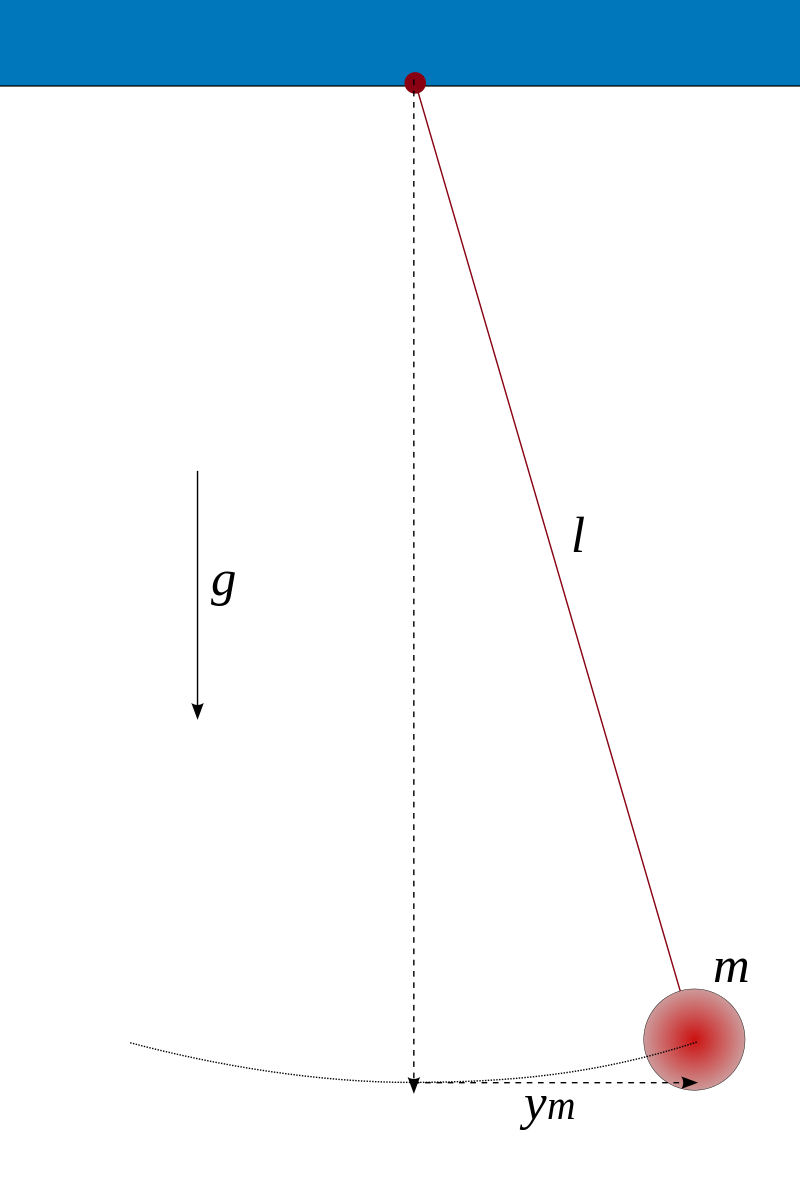
\includegraphics[scale=0.2]{Pendulum.png}
  \caption{Pendule simple}
  \label{fig:pendule simple}
\end{figure}
Lorsque le pendule est écarté de sa position d'équilibre (la verticale), son point matériel de masse m se déplace le long d'un arc de cercle sous l'effet de son poids, qui le ramène constamment vers sa position d'équilibre.\\
Le problème posé consiste à prédire la position du pendule dans le temps en connaissant sa masse $m$, la longueur $l$ du fil, et l'angle de départ $\theta_0$ formé par le fil avec la verticale (on supposera que la vitesse angulaire initiale est nulle). Connaître l'angle $\theta$ que forme le pendule à différents moments dans le temps permettra donc de résoudre ce problème. On supposera par la suite que $\theta$ est deux fois dérivable (cela a un sens en mécanique classique).

\subsection{Mise en équation}
Pour établir l'équation du problème, nous allons utiliser le concept d'énergie mécanique du pendule simple.\\
L'énergie mécanique totale du pendule simple à l'instant $t$ est donnée par :
\[ E_{\text{tot}}(t) = E_{\text{c}}(t) +  E_{\text{p}}(t) \Leftrightarrow E_{\text{tot}}(t) = \frac{1}{2}m(l\theta'(t))^2 + mgl(1 - \cos(\theta(t))) \]
En considérant la conservation de l'énergie mécanique ($E_{\text{tot}}$ reste constant), nous pouvons établir l'équation différentielle du mouvement du pendule simple :
\[E_{\text{tot}}'(t) = 0 \Leftrightarrow \theta''(t) = -\frac{g}{l}\sin(\theta(t))\]
Cette équation décrit l'évolution de l'angle $\theta$ du pendule en fonction du temps $t$.
\begin{tcolorbox}
    \begin{rem}
        Il existe d'autres méthodes pour aboutir à cette équation, comme l'application du principe fondamental de la dynamique, ou l'application du théorème du moment cinétique.
    \end{rem}
\end{tcolorbox}

\subsection{Etude qualitative}
Pour étudier l'équation différentielle, on commence par réécrire l'équation sous la forme d'un problème de Cauchy.\\
Posons $X(t) = \begin{pmatrix}\theta(t) \\\theta'(t) \\\end{pmatrix}$, pour tout $t\geq0$
\\On a donc aussi : $X'(t) = \begin{pmatrix}\theta'(t) \\\theta''(t) \\\end{pmatrix} = \begin{pmatrix}\theta'(t) \\\frac{-g}l sin(\theta(t)) \\\end{pmatrix}$
\\En notant $f$ la fonction définie par $\begin{cases}
  \mathbb{R} \times \mathbb{R}^2 \longrightarrow \mathbb{R}^2\\
  (t,y=(y_1,y_2)) \longmapsto \begin{pmatrix}y_2 \\\frac{-g}l sin(y_1) \end{pmatrix} \end{cases}$

$\\$ On a alors que : $X'(t)=f(t,X(t))$, pour tout $t \geq 0$
\\ L'équation devient donc :
$$
\begin{cases} 
X'(t) = f(t,X(t)) & \forall t \geq 0 \\
X(0)=\begin{pmatrix}
    \theta_0\\
    0
\end{pmatrix} := X_0
\end{cases}
$$
\subsubsection{Existence d'une unique solution maximale}
Vérifions maintenant que l'équation différentielle admet une solution et montrons que la solution est unique.
\\Puisqu'il s'agit d'un problème de Cauchy, appliquons le théorème de Cauchy-Lipschitz maximal :
\begin{itemize}[label=\textbullet]
    \item $f$ est continue : $\mathbb{R} \times \mathbb{R}^2 \rightarrow \mathbb{R}$
    \item $\frac{\partial f_1}{\partial y_1}$ : 
    $\begin{cases}
        \mathbb{R} \times \mathbb{R}^2 \rightarrow \mathbb{R} \\
        (t,y=(y_1,y_2)) \mapsto 0
    \end{cases}$ est continue sur $\mathbb{R} \times \mathbb{R}^2$
    \item $\frac{\partial f_1}{\partial y_2}$ : 
    $\begin{cases}
        \mathbb{R} \times \mathbb{R}^2 \rightarrow \mathbb{R} \\
        (t,y=(y_1,y_2)) \mapsto 1
    \end{cases}$est continue sur $\mathbb{R} \times \mathbb{R}^2$
    \item $\frac{\partial f_2}{\partial y_1}$ : 
    $\begin{cases}
        \mathbb{R} \times \mathbb{R}^2 \rightarrow \mathbb{R} \\
        (t,y=(y_1,y_2)) \mapsto \frac{-g}l cos(y_1)
    \end{cases}$est continue sur $\mathbb{R} \times \mathbb{R}^2$
    \item $\frac{\partial f_2}{\partial y_2}$ : 
    $\begin{cases}
        \mathbb{R} \times \mathbb{R}^2 \rightarrow \mathbb{R} \\
        (t,y=(y_1,y_2)) \mapsto 0
    \end{cases}$ est continue sur $\mathbb{R} \times \mathbb{R}^2$
\end{itemize}
Par le théorème de Cauchy-Lipschitz, il existe une unique solution maximale $y^*:=\begin{pmatrix}
    y_1\\
    y_2
\end{pmatrix}$ sur $[0,T^*[$, pour un certain $T^* > 0$, du problème de Cauchy. Cette solution est donc $X = \begin{pmatrix}
    \theta\\
    \theta'
\end{pmatrix}$.\\
\subsubsection{Existence d'une unique solution globale}
On se demande maintenant si $T^* = +\infty$, c'est à dire si la solution maximal est globale ?\\
Pour répondre à cette question, il suffit de remarquer que :
\begin{tcolorbox}[colback=green!5!white, colframe=green!50!black]
    $$
    \forall(t,y) \in \mathbb{R}_+ \times \mathbb{R}^2, \|f(t,y)\|_\infty \leq \frac{g}{l} + \|y\|_\infty
    $$
    où $\|y\|_\infty = max(|y_1|,|y_2|)$.
\end{tcolorbox}
En effet, soit $(t,y) \in \mathbb{R}_+ \times \mathbb{R}^2$. $\|f(t,y)\|_\infty = \max(|y_2|,\frac{g}{l}|sin(y_1)|) \leq \max(|y_2|,\frac{g}{l})$.\\
Par disjonction de cas, on a :
\begin{itemize}[label=\textbullet]
    \item Si $|y_2| \leq \frac{g}{l}$, alors $\max(|y_2|,\frac{g}{l}) = \frac{g}{l} \leq \frac{g}{l} + \|y\|_\infty$.
    \item Si $\frac{g}{l} \textless |y_2|$, alors $\max(|y_2|,\frac{g}{l}) = |y_2| \leq \frac{g}{l} + \max(|y_1|,|y_2|) = \frac{g}{l} + \|y\|_\infty$.
\end{itemize} 
Donc $\|f(t,y)\|_\infty \leq \max(|y_2|, \frac{g}{l}) \leq \frac{g}{l} + \|y\|_\infty$.\\
Par une proposition de cours, la solution est globale donc définie sur $\mathbb{R}_+$.\\\\
Néanmoins, il n'existe pas, pour le moment, d'expression de la solution (on peut aboutir à une expression si on avait linéarisé l'équation : $\theta''(t)+\frac{g}{l}\theta(t) = 0, \forall t \geq 0$ en utilisant l'approximation des petits angles, c'est à dire : $\sin(\theta(t)) \approx \theta(t)$).\\
On va donc utiliser la méthode de RK4 pour approcher numériquement la solution.
\begin{tcolorbox}
    \begin{rem}
        On se doutait de l'existence d'une solution par la nature physique du problème. En effet, par l'absurde, si l'équation n'admettait pas de solutions, alors la fonction $\theta$ représentant l'angle ne pourrait pas vérifier l'équation, donc cela remettrait en question les lois de la mécanique classique, ce qui est absurde pour un problème aussi simple que celui du pendule simple d'où son nom...
    \end{rem}
\end{tcolorbox}
\subsubsection{Intégrale première du mouvement (en physique)}
Maintenant qu'on sait qu'une unique solution globale existe, étudions la.\\
Pour cela, nous allons avoir besoin d'intégrer l'\gls{edo} :
$$
\left\{
  \begin{array}{lcl}
    \theta''(t) + \frac{g}{l}\sin(\theta(t)) = 0, & \forall t \geq 0 \\
    \theta(0) = \theta_0 \in ]-\pi, \pi] \\
    \theta'(0) = 0 \\
  \end{array}
\right.
$$
ou encore, en multipliant par $2\theta'(t)$ de part et d'autre de l'égalité :
$$
\left\{
  \begin{array}{lcl}
    2\theta'(t)\theta''(t) = \frac{-2g}{l}\sin(\theta(t))\theta'(t), & \forall t \geq 0 \\
    \theta(0) = \theta_0 \in ]-\pi, \pi] \\
    \theta'(0) = 0 \\
  \end{array}
\right.
$$
On obtient alors :
$$
\int_0^t2\theta'(x)\theta''(x)dx = \int_0^t\frac{-2g}{l}\sin(\theta(x))\theta'(x)dx, \forall t \geq 0
$$
c'est-à-dire :
$$
[(\theta'(x))^2]_0^t = \frac{2g}{l}[\cos(\theta(x))]_0^t, \forall t \geq 0
$$
ou encore :
\begin{tcolorbox}[colback=green!5!white, colframe=green!50!black]
    $$
    [\theta'(t)]^2 = \frac{2g}{l}[\cos(\theta(t)) - \cos(\theta_0)], \forall t \geq 0
    $$
\end{tcolorbox}
Vous avez devant vous l'intégrale première du mouvement en physique.\\
De cette équation, on tire deux informations :
\begin{itemize}[label=\textbullet]
    \item $\forall t \geq 0, \theta'(t) = 0 \Leftrightarrow \cos(\theta(t)) = \cos(\theta_0) \Leftrightarrow \exists k \in \mathbb{Z}, \theta(t) = \theta_0 + 2k\pi \lor \theta(t) = -\theta_0 + 2k\pi$ : vitesse nulle seulement aux extrémités du pendule (on y reviendra)
    \item $\forall t \geq 0, \cos(\theta(t)) \geq \cos(\theta_0)$ : solution bornée (on y reviendra aussi)
\end{itemize}
\subsubsection{Solution constante}
On se demande à quelle condition nécessaire et suffisante sur $\theta_0$ la solution est-elle constante ?\\
Pour cela, on va s'intéresser aux équilibres de l'\gls{edo} (sans prendre en compte les conditions initiales) :\\
Soit $y = \begin{pmatrix}
    y_1 \\
    y_2
\end{pmatrix} \in \mathbb{R}^2$.\\\\
$y$ est solution de l'\gls{edo} (sans prendre en compte les conditions initiales) ssi $f(t, y) = \begin{pmatrix}
    0 \\
    0
\end{pmatrix}$, pour tout $t \geq 0$ ssi $\begin{pmatrix}
    y_2 \\
    -\frac{g}{l}\sin(y_1)
\end{pmatrix} = \begin{pmatrix}
    0 \\
    0
\end{pmatrix}$ ssi $\left\{
  \begin{array}{lcl}
    y_1 = k\pi, \text{ pour un certain $k \in \mathbb{Z}$} \\
    y_2 = 0 \\
  \end{array}
\right.$\\\\\\
Ainsi, par unicité de la solution du problème de Cauchy,
\begin{itemize}[label=\textbullet]
    \item Si $\theta_0 = 0$, alors $\theta(t) = 0$, pour tout $t \geq 0$
    \item Si $\theta_0 = \pi$, alors $\theta(t) = \pi$, pour tout $t \geq 0$
\end{itemize}
Par ailleurs, ce sont les deux seules situations où la solution est constante, d'après l'équivalence qu'on vient de montrer.
\subsubsection{Solution bornée}
Supposons à présent que $\theta_0 \notin \{0, \pi\}$.\\
La solution est-elle bornée ? La réponse est oui. On va montrer que :
\begin{tcolorbox}[colback=green!5!white, colframe=green!50!black]
    $$
    \forall t \geq 0, -|\theta_0| \leq \theta(t) \leq |\theta_0|
    $$
\end{tcolorbox}
\textbf{\textit{Preuve}} : Raisonnons par l'absurde. Supposons par l'absurde que $(\forall t \geq 0, -|\theta_0| \leq \theta(t) \leq |\theta_0|)$ est faux, autrement dit que $(\exists t \geq 0, \theta(t) < -|\theta_0| \lor \theta(t) > |\theta_0|)$ est vraie.\\
\begin{itemize}[label=\textbullet]
    \item Commençons par le cas où il existe $t_1 \geq 0$ tel que $\theta(t_1) > |\theta_0|$. Faisons une disjonction de cas :
    \begin{itemize}[label=\textbullet]
        \item Si $\theta(t_1) \leq \pi$, alors on a $0 < |\theta_0| < \theta(t_1) \leq \pi$, donc, par strict. décroissance de la fonction cos sur $[0, \pi]$, $-1 \leq \cos(\theta(t_1)) < \cos(|\theta_0|) < 1$, donc $\cos(\theta(t_1)) < \cos(\theta_0)$.
        \item Si $\theta(t_1) > \pi$, puisque $\theta(0) = \theta_0 < \pi$, par le TVI ($\theta$ est continue sur $\mathbb{R}_+$), il existe $t_2 \in [0, t_1]$ tel que $\theta(t_2) = \pi$. Donc $0 < |\theta_0| < \pi = \theta(t_2)$ et donc, par strict. décroissance de la fonction cos sur $[0, \pi]$, $\cos(\theta(t_2)) < \cos(|\theta_0|) < 1$, donc $\cos(\theta(t_2)) < \cos(|\theta_0|)$.
    \end{itemize}
    Dans les deux cas, $(\exists t \geq 0, \cos(\theta(t)) < \cos(\theta_0))$ est vraie, ce qui est absurde car $(\forall t \geq 0, \cos(\theta(t)) \geq \cos(\theta_0))$ est vraie, d'après l'intégrale première du mouvement.
    \item Trouver l'absurdité pour le cas où il existe $t_1 \geq 0$ tel que $\theta(t_1) < -|\theta_0|$ est laissé au lecteur ; le raisonnement est très similaire.
\end{itemize}
Ainsi, on a montré le résultat voulu.
\subsubsection{Variations de la solution}
La solution est-elle croissante ? décroissante ? les deux ? Nous allons répondre à ces question ci-dessous.\\
Supposons tout d'abord que $\theta_0 > 0$. Nous allons montrer le résultat suivant :
\begin{tcolorbox}[colback=green!5!white, colframe=green!50!black]
    \begin{prop}
        Si $\theta_0 > 0$, alors $\theta$ est strictement décroissante de $\theta_0$ à $-\theta_0$ sur $[0, \tilde{T}]$ et strictement croissante de $-\theta_0$ à $\theta_0$ sur $[\tilde{T}, 2\tilde{T}]$, pour un certain $\tilde{T} > 0$.
    \end{prop}
\end{tcolorbox}
\textbf{\textit{Preuve}} :
\begin{itemize}[label=\textbullet]
    \item Commençons par montrer que $\theta$ est strictemement décroissante de $\theta_0$ à $-\theta_0$ sur $[0, \tilde{T}]$.
    \begin{itemize}[label=\textbullet]
        \item Tout d'abord, on va exclure le cas où $\theta$ est décroissante sur $\mathbb{R}_+$ en raisonnant par l'absurde et donc supposons par l'absurde que $\theta$ est décroissante sur $\mathbb{R}_+$.\\
        Puisque $\theta$ est une fonction bornée, alors $\theta$ converge vers un certain $\theta_l \in [-\theta_0, \theta_0[ \subset ]-\pi, \pi[$.\\
        De plus, par l'intégrale première du mouvement, puisque $[\theta'(t)]^2 = \frac{2g}{l}[\cos(\theta(t)) - \cos(\theta_0)]$, pour tout $t \geq 0$, alors $\theta'$ converge vers $-\sqrt{\frac{2g}{l}[\cos(\theta_l) - \cos(\theta_0)]}$ ($\theta$ est décroissante sur $\mathbb{R}_+$ donc $\theta' \leq 0$). Par une proposition (voir annexe) que j'ai démontré, alors nécessairement $-\sqrt{\frac{2g}{l}[\cos(\theta_l) - \cos(\theta_0)]} = 0$, autrement dit $\theta_l = -\theta_0$ (car $\theta_l \neq \theta_0$ et $\theta_l \in ]-\pi, \pi[$).\\
        Par ailleurs, puisque $\theta''(t) = \frac{-g}{l}\sin(\theta(t))$, pour tout $t \geq 0$, alors $\theta''$ converge vers $\frac{-g}{l}\sin(\theta_l)$. Par la même proposition appliqueée à la fonction $\theta'$, nécessairement $\frac{-g}{l}\sin(\theta_l) = 0$, c'est-à-dire $\theta_l = 0$ (car $\theta_l \in ]-\pi, \pi[$ et $\sin(\theta_l) = 0$).\\
        Par conséquent, on a montré que $\theta_l = -\theta_0 \neq 0$ et $\theta_l = 0$, ce qui est absurde.
        \item Maintenant qu'on a exclut ce cas, on peut commencer.
        \begin{itemize}[label=\textbullet]
            \item On remarque que $\theta''(0) = \frac{-g}{l}\sin(\theta_0) < 0$ (car $\theta_0 \in ]0, \pi[$). Par continuité de $\theta''$ sur $\mathbb{R}_+$, il existe $\tilde{\eta} > 0$ tel que, pour tout $t \in [0, \tilde{\eta}]$, $\theta''(t) < 0$, donc sur $[0, \tilde{\eta}]$, $\theta'$ est strictement décroissante. Or, $\theta'(0) = 0$. Par conséquent, pour tout $t \in [0, \tilde{\eta}]$, $\theta'(t) \leq 0$ et donc $\theta$ est décroissante sur $[0, \tilde{\eta}]$ (encore mieux, $\theta$ est strictement décroissante sur $[0, \tilde{\eta}]$ car $\theta'(t) = 0$ seulement pour $t = 0$).
            \item On peut alors poser $\tilde{T} := \sup(A)$, avec $A := \{\eta > 0 : \forall t \in ]0, \eta], \theta'(t) < 0\}$.\\
            En effet, $A$ est une partie non vide de $\mathbb{R}$ car $\tilde{\eta} \in A$ (donc $\tilde{T} > 0$) et c'est une partie bornée de $\mathbb{R}$ car sinon, cela voudrait dire que $\theta$ est strictement décroissante sur $\mathbb{R}_+$ ; cas qu'on a exclut.
            \item Montrons d'abord que $A$ est un ouvert de $\mathbb{R}$.\\
            Soit $\eta \in A$. Alors, pour tout $t \in ]0, \eta]$, $\theta'(t) < 0$. En particulier, $\theta'(\eta) < 0$. Par continuité de $\theta'$ sur $\mathbb{R}_+$, il existe $\epsilon > 0$ tel que $\eta - \epsilon \geq 0$ et, pour tout $t \in ]\eta - \epsilon, \eta + \epsilon[$, $\theta'(t) < 0$. En somme, pour tout $t \in ]0, \eta + \epsilon[$, $\theta'(t) < 0$, donc $]\eta - \epsilon, \eta + \epsilon[ \subset A$, d'où $A$ est un ouvert de $\mathbb{R}$.
            \item Montrons à présent que $A = ]0, \tilde{T}[$.\\
            En effet, $A \subset ]0, \tilde{T}[$ (car $A \subset ]0, \tilde{T}]$ et $A$ est un ouvert de $\mathbb{R}$ donc $\tilde{T} \notin A$). Pour l'inclusion inverse, soit $t_1 \in ]0, \tilde{T}[$. Puisque $\tilde{T}$ est le plus petit des majorants de $A$, alors $t_1$ n'est pas un majorant de $A$, et donc il existe $t_2 > t_1$ tel que $t_2 \in A$. Donc pour tout $t \in ]0, t_2]$, $\theta'(t) < 0$, en particulier, pour tout $t \in ]0, t_1]$, $\theta'(t) < 0$, autrement dit $t_1 \in A$, d'où $]0, \tilde{T}[ \subset A$.
            \item On vient donc de montrer que :
            $$
            \forall t \in ]0, \tilde{T}[, \theta'(t) < 0
            $$
            \item Montrons enfin que $\theta'(\tilde{T}) = 0$.\\
            En effet, puisque $\tilde{T}$ est le plus petit des majorants de $A$, on peut construire une suite $(\eta_n)_{n \in \mathbb{N}}$ d'éléments de $A$ qui converge vers $\tilde{T}$. Par conséquent, puisque, pour tout $n \in \mathbb{N}$, $\theta'(\eta_n) < 0$ et par continuité de $\theta'$ sur $\mathbb{R}_+$, on a :
            $$
            \theta'(\tilde{T}) = \lim_{n \to +\infty}\theta'(\eta_n) \leq 0
            $$
            Or, $\theta'(\tilde{T}) < 0$ n'est pas possible. En effet, par l'absurde, si c'était le cas, alors on aurait :
            $$
            \forall t \in ]0, \tilde{T}], \theta'(t) < 0
            $$
            autrement dit $\tilde{T} \in A$, ce qui est absurde car $\tilde{T} \notin A$. D'où $\theta'(\tilde{T}) = 0$.
            \item On a donc montré que :
            $$
            \left\{
            \begin{array}{lcl}
                \theta'(t) < 0, & \forall t \in ]0, \tilde{T}[ \\
                \theta'(0) = \theta'(\tilde{T}) = 0 \\
            \end{array}
            \right.
            $$
            et donc :
            $$
            \left\{
            \begin{array}{lcl}
                \theta'(t) < 0, & \forall t \in ]0, \tilde{T}[ \\
                \theta(0) = \theta_0, \theta(\tilde{T}) = -\theta_0 \\
                \theta'(0) = \theta'(\tilde{T}) = 0 \\
            \end{array}
            \right.
            $$
            car $\theta'(\tilde{T}) = 0$ et $\theta(\tilde{T}) \neq \theta_0$ (car $\theta(0) = \theta_0$ et $\theta$ est strictement décroissante sur $]0, \tilde{T}[$) donc, d'après l'intégrale première du mouvement, $\theta(\tilde{T}) = -\theta_0$.
        \end{itemize}
    \end{itemize}
    Ainsi, on a montré que $\theta$ est strictement décroissante de $\theta_0$ à $-\theta_0$ sur $[0, \tilde{T}]$ (et la vitesse angulaire est nulle seulement lorsque $\theta$ vaut $-\theta_0$ ou $\theta_0$).
    \item Montrons à présent que $\theta$ est croissante de $-\theta_0$ à $\theta_0$ sur $[\tilde{T}, 2\tilde{T}]$.\\
    Posons, pour tout $t \geq 0$, $\tilde{\theta}(t) = -\theta(t + \tilde{T})$.
    \begin{itemize}[label=\textbullet]
        \item $\tilde{\theta}(0) = -\theta(\tilde{T}) = -(-\theta_0) = \theta_0$ et $\tilde{\theta}'(0) = -\theta'(\tilde{T}) = 0$
        \item $\tilde{\theta}''(t) = -\theta''(t + \tilde{T}) = -[\frac{-g}{l}\sin(\theta(t + \tilde{T}))] = \frac{-g}{l}\sin(-\theta(t + \tilde{T})) = \frac{-g}{l}\sin(\tilde{\theta}(t))$, pour tout $t \geq 0$
    \end{itemize}
    Donc $\tilde{\theta}$ est aussi une solution du problème de Cauchy. Par unicité de la solution, $\tilde{\theta} = \theta$, autrement dit $-\theta(t + \tilde{T}) = \theta(t)$, pour tout $t \geq 0$, c'est-à-dire $\theta(t) = -\theta(t - \tilde{T})$, pour tout $t \geq \tilde{T}$.\\
    Or,
    \begin{itemize}[label=\textbullet]
        \item $t \longmapsto t - \tilde{T}$ est strictement croissante sur $[\tilde{T}, 2\tilde{T}]$ à valeurs dans $[0, \tilde{T}]$.
        \item $u \longmapsto \theta(u)$ est strictement décroissante sur $[0, \tilde{T}]$ à valeurs dans $[-\theta_0, \theta_0]$.
        \item $v \longmapsto -v$ est strictement décroissante sur $[-\theta_0, \theta_0]$ à valeurs dans $[-\theta_0, \theta_0]$.
    \end{itemize}
    Ainsi, par composition de fonctions, $\theta$ est strictement croissante sur $[\tilde{T}, 2\tilde{T}]$ à valeurs dans $[-\theta_0, \theta_0]$, $\theta(\tilde{T}) = -\theta_0$ et $\theta(2\tilde{T}) = -\theta(2\tilde{T} - \tilde{T}) = -\theta(\tilde{T}) = \theta_0$ ; $\theta$ est donc strictement croissante de $-\theta_0$ à $\theta_0$ sur $[\tilde{T}, 2\tilde{T}]$.
\end{itemize}
\begin{tcolorbox}
    \begin{rem}
        L'intuition que j'ai eu (pour montrer la stric. croissance) provient de la symétrie du problème du pendule simple. En effet, lorsque le pendule a un angle de $-\theta_0$ et une vitesse angulaire nulle, c'est la même configuration que celle initiale si on se place de l'autre côté du pendule. Ce "changement de côté" se manifeste dans les calculs par le signe $-$ et le "$t + \tilde{T}$" signifie qu'on se place $\tilde{T}$ de temps plus tard, c'est-à-dire une fois que le pendule a atteint l'angle $-\theta_0$.
    \end{rem}
\end{tcolorbox}
Supposons maintenant que $\theta_0 < 0$.\\
On a alors le résultat suivant :
\begin{tcolorbox}[colback=green!5!white, colframe=green!50!black]
    \begin{prop}
        Si $\theta_0 < 0$, alors $\theta$ est strictement croissante de $\theta_0$ à $-\theta_0$ sur $[0, \tilde{T}]$ et strictement décroissante de $-\theta_0$ à $\theta_0$ sur $[\tilde{T}, 2\tilde{T}]$
    \end{prop}
\end{tcolorbox}
\begin{tcolorbox}
    \begin{rem}
        En réalité, tout comme pour la remarque précédente, le cas où $\theta_0 < 0$ est le même que le cas où $\theta_0 > 0$ si on se place de l'autre côté du pendule. Ayons la même intuition que tout-à-l'heure.
    \end{rem}
\end{tcolorbox}
\textbf{\textit{Preuve}} : Posons $\tilde{\theta} = -\theta$.
\begin{itemize}[label=\textbullet]
    \item $\tilde{\theta}(0) = -\theta_0 > 0$ et $\tilde{\theta}'(0) = -\theta'(0) = 0$
    \item $\tilde{\theta}''(t) = -\theta''(t) = \frac{-g}{l}\sin(-\theta(t)) = \frac{-g}{l}\sin(\tilde{\theta}(t))$, pour tout $t \geq 0$
\end{itemize}
 Donc $\tilde{\theta}$ est solution du problème de Cauchy avec comme données initiales $\tilde{\theta}(0) = -\theta_0 > 0$ et $\tilde{\theta}'(0) = 0$. Par la proposition, $\tilde{\theta}$ est strictement décroissante de $-\theta_0$ à $\theta_0$ sur $[0, \tilde{T}]$ et strictement croissante de $\theta_0$ à $-\theta_0$ sur $[\tilde{T}, 2\tilde{T}]$ (il s'agit du même $\tilde{T}$ que précédemment) et ainsi, $\theta = -\tilde{\theta}$ est strictement croissante de $\theta_0$ à $-\theta_0$ sur $[0, \tilde{T}]$ et strictement décroissante de $-\theta_0$ à $\theta_0$ sur $[\tilde{T}, 2\tilde{T}]$.
 \begin{tcolorbox}
     \begin{rem}
        L'antisymétrie du problème est mise en lumière par l'imparité de la fonction sinus dans l'\gls{edo}.
    \end{rem}
 \end{tcolorbox}
\subsubsection{Solution périodique}
Lorsqu'on pense au pendule simple, on pense de suite à sa période (mouvement qui oscille). Cela voudrait dire que la solution est périodique ?\\
Pour cela, nous allons d'abord montrer le résultat général suivant :
\begin{tcolorbox}[colback=green!5!white, colframe=green!50!black]
    \begin{prop}
        On considère le problème de Cauchy :
        $$
        \left\{
    \begin{array}{lcl}
        y'(t) = f(t, y(t)), & \forall t \geq 0 \\
        y(0) = y^0 \in \mathbb{R}^d
    \end{array}
    \right.
        $$
        où $f : \mathbb{R} \times \mathbb{R}^d \longrightarrow \mathbb{R}^d$ et $y^0 \in \mathbb{R}^d$ sont les données du problème vérifiant les hypothèses du théorème de Cauchy-Lipschitz global.\\
        Supposons que l'équation est autonome (i.e. pour tout $(t, y) \in \mathbb{R} \times \mathbb{R}^d$, $f(t, y) = g(y)$ pour une certaine fonction $g$) et qu'il existe $T > 0$ tel que $y(T) = y^0$.\\
        Alors :
        $$
        y(t + T) = y(t), \forall t \geq 0
        $$
    \end{prop}
\end{tcolorbox}
\textbf{\textit{Preuve}} : Posons, pour tout $t \geq 0$, $z(t) = y(t + T)$.
\begin{itemize}[label=\textbullet]
    \item $z(0) = y(T) = y^0$
    \item $z'(t) = y'(t + T) = f(t + T, y(t + T)) = g(y(t + T)) = g(z(t)) = f(t, z(t))$, pour tout $t \geq 0$
\end{itemize}
$z$ est donc solution du problème de Cauchy tout comme $y$. Par unicité de la solution, $z = y$, autrement dit :
$$
y(t + T) = y(t), \forall t \geq 0
$$
Ainsi, en remarquant que $f$ est bien autonome et que $\theta(2\tilde{T}) = \theta_0$ et $\theta'(2\tilde{T}) = 0$ (quelque soit le signe de $\theta_0$), c'est-à-dire $X(2\tilde{T}) = X_0$, alors, d'après la proposition qu'on vient de montrer, $\theta$ et $\theta'$ sont $2\tilde{T}$-périodique.
\subsection{Etude numérique}
Dans cette section, nous allons en réalité approcher numériquement $\theta$ et $\theta'$ puisque l'\gls{edo} doit être mise sous forme d'un problème de Cauchy pour utiliser la méthode de \gls{rk4}.\\
Ici,
$$
f(t, y) = \begin{pmatrix}
    y_2\\
    -\frac{g}{l}\sin(y_1)
\end{pmatrix}, \forall (t, y) \in \mathbb{R} \times \mathbb{R}^2
$$
On peut donc compléter le fichier f.c :
\begin{Verbatim}[numbers=left, frame=single]
#include "vecteur.h"
#include <math.h>
#include "f.h"

extern double l;

Vecteur_t f(double t, Vecteur_t y) // d = 2
{
    Vecteur_t z;
    z.d = y.d;
    z.x[0] = y.x[1];
    z.x[1] = -g/l*sin(y.x[0]);

    return z;
}
\end{Verbatim}
La ligne 5 permet d'éviter de passer l en paramètre de la fonction f afin d'avoir juste à modifier le contenu de la fonction f si le problème change et non tous les prototypes, les pointeurs de fonctions et appels à la fonction f, ... Il faut voir l comme un paramètre et non une variable à part entière de f.\\\\
On a ensuite créé un fichier recuperation\_donnees.c qui comme l'indique le nom, permettra de récupérer les données du problème par l'utilisateur (le temps final $T$ en secondes, le nombre d'intervalles $N$ pour la discrétisation, l'angle initial $\theta_0$ en radians et la longueur $l$ de la tige en mètres). On ne demande pas la masse de la bille car comme on l'a expliqué, le mouvement du pendule simple ne dépend pas de la masse de la bille. Il faudra exécuter le programme recuperation\_donnees.exe pour récupérer les données.\\\\
Les données sont ensuite stockés dans le fichier donnees\_entree.txt sous le format suivante :
\begin{Verbatim}
T l theta_0 N
\end{Verbatim}
Par exemple :
\begin{Verbatim}
20 1 1 600
\end{Verbatim}
Ensuite, on a créé le fichier calcul\_solution.c qui récupère les données, calcule une approximation de $\theta$ et $\theta'$ selon la méthode de \gls{rk4} (donc appel de la fonction runge\_kutta\_4 avec la fonction f en paramètre) puis il écrit la solution dans le fichier donnees\_sortie.txt sous le format suivant :
\begin{Verbatim}
t_0 theta_0
t_1 theta_1
.
.
.
t_N theta_N
\end{Verbatim}
On ne récupère donc pas l'approximation de $\theta'$, on n'en a pas besoin pour la simulation. Il faudra exécuter le programme calcul\_solution.exe pour effectuer les tâches décrites.\\\\
Enfin, le fichier simulation\_pendule\_simple.py récupère l'approximation et les données du problème et réalise une simulation à partir de celles-ci. L'utilisation du langage python est justifiée par la simplicité du module pygame permettant des affichages graphiques.\\\\
Pour la compilation, on a réalisé un makefile. Il suffira donc de taper :
\begin{Verbatim}
    make recuperation_donnees.exe
\end{Verbatim}
pour créer l'exécutable recuperation\_donnees.exe et :
\begin{Verbatim}
    make calcul_solution.exe
\end{Verbatim}
pour créer l'exécutable calcul\_solution.exe.
\section{Pendule couplé}
\subsection{Définition et histoire}
Le pendule couplé est un autre problème physique qui est constitué de deux pendules simples couplé avec un ressort.\\
Dans ce nouveau système on considère, en plus des deux pendules, le ressort qui rajoute une force supplémentaire à considérer dans notre étude de ce problème.\\
On supposera que les deux pendules sont de longueur $l$, et que le ressort, de raideur $k$, est fixé de chaque côté sur les pendules à une distance de $a$ par rapport à l'axe de rotation de chaque pendule. On notera respectivement $m_1$ et $m_2$ les masses ponctuelles du premier et deuxième pendule et $\theta_1$ et $\theta_2$ les angles formés avec la verticale du premier et deuxième pendule (on supposera que la vitesse angulaire initiale des deux pendules est nulle).
\subsection{Mise en équation}
On remarque alors que déterminer les angles $\theta_1$ et $\theta_2$ à tout instant permettra de connaître le mouvement du pendule couplé et donc de résoudre ce problème.\\
Le calcul du moment des forces par rapport aux axes de rotation et l'application du théorème du moment cinétique permettent d'établir les équations du mouvement que vérifient $\theta_1$ et $\theta_2$ :
$$
\left\{
\begin{array}{lcl}
    m_1l^2\theta_1''(t) + m_1gl\sin(\theta_1(t)) - a^2k(\sin(\theta_2(t)) - \sin(\theta_1(t)))\cos(\theta_1(t)) = 0, & \forall t \geq 0 \\
    m_2l^2\theta_2''(t) + m_2gl\sin(\theta_2(t)) + a^2k(\sin(\theta_2(t)) - \sin(\theta_1(t)))\cos(\theta_2(t)) = 0, & \forall t \geq 0 \\
\end{array}
\right.
$$
c'est-à-dire :
$$
\left\{
\begin{array}{lcl}
    \theta_1''(t) = \frac{a^2k(sin(\theta_2(t))-sin(\theta_1(t)))cos(\theta_1(t))-m_1glsin(\theta_1(t))}{m_1l^2}, & \forall t \geq 0 \\
    \theta_2''(t) = \frac{-a^2k(sin(\theta_2(t))-sin(\theta_1(t)))cos(\theta_2(t))-m_2glsin(\theta_2(t))}{m_2l^2}, & \forall t \geq 0 \\
\end{array}
\right.
$$
Ce système d'équations décrit l'évolution des angles $\theta_1$ et $\theta_2$ des pendules en fonction du temps.
\subsection{Etude qualitative}
Pour étudier ce système d'EDO, on commence par écrire l'équation sous la forme d'un problème de Cauchy.\\
Posons $X(t)=\begin{pmatrix}
    \theta_1(t)\\
    \theta_2(t)\\
    \theta_1'(t)\\
    \theta_2'(t)
\end{pmatrix}$ pour tout t$\geq$0\\
On a aussi : $X'(t)=\begin{pmatrix}
    \theta_1'(t)\\
    \theta_2'(t)\\
    \theta_1''(t)\\
    \theta_2''(t)
\end{pmatrix}$ pour tout t$\geq$0\\
Or d'après les équations de mouvement :
\\$X'(t) = \begin{pmatrix}
    \theta_1'(t)\\
    \theta_2'(t)\\
    \frac{a^2k(sin(\theta_2)-sin(\theta_1))cos(\theta_1)-m_1glsin(\theta_1)}{m_1l^2}\\
    \frac{a^2k(sin(\theta_2)-sin(\theta_1))cos(\theta_2)-m_1glsin(\theta_1)}{m_2l^2}
\end{pmatrix}$\\
On note donc $f$ la fonction définie par : \begin{cases}
    $$
    \mathbb{R} \times \mathbb{R}^4 \longrightarrow \mathbb{R}^4\\
    (t,y=(y_1,y_2,y_3,y_4)) \longmapsto \begin{pmatrix}
    y_3\\
    y_4\\
    \frac{a^2k(sin(y_2)-sin(y_1))cos(y_1)-m_1glsin(y_1)}{m_1l^2}\\
    \frac{a^2k(sin(y_2)-sin(y_1))cos(y_2)-m_1glsin(y_1)}{m_2l^2}
    \end{pmatrix}
    $$
\end{cases}\\
On a alors : $X'(t) = f(t,X(t))$, pour tout $t \geq 0$\\
L'équation devient donc : \begin{cases}
    $$
    X'(t) = f(t,X(t)), & \forall t \geq 0\\
    X(0) = \begin{pmatrix}
    \theta_{1,0}\\
    \theta_{2,0}\\
        0\\
        0
    \end{pmatrix} := X_0
    $$
\end{cases}
\begin{figure}
  \centering
  \includegraphics[scale=0.9]{Double_pendule.png}
  \caption{Pendule couplé}
  \label{fig:pendule couplé}
\end{figure}
\subsubsection{Existence d'une solution maximale}
Vérifions maintenant que l'équation différentielle admet une solution et montrons que la solution est unique.
\\Puisqu'il s'agit d'un problème de Cauchy, appliquons le théorème de Cauchy-Lipschitz maximal :
\begin{itemize}[label=\textbullet]
    \item $f$ est continue : $\mathbb{R} \times \mathbb{R}^4 \rightarrow \mathbb{R}$
    
    \item $\frac{\partial f_1}{\partial y_1} = \frac{\partial f_1}{\partial y_2} =\frac{\partial f_1}{\partial y_4}$ : 
    $\begin{cases}
        \mathbb{R} \times \mathbb{R}^4 \rightarrow \mathbb{R} \\
        (t,y=(y_1,y_2,y_3,y_4)) \mapsto 0
    \end{cases}$ sont continues sur $\mathbb{R} \times \mathbb{R}^4$
    
    \item $\frac{\partial f_1}{\partial y_3}$ : 
    $\begin{cases}
        \mathbb{R} \times \mathbb{R}^4 \rightarrow \mathbb{R} \\
        (t,y=(y_1,y_2,y_3,y_4)) \mapsto 1
    \end{cases}$est continue sur $\mathbb{R} \times \mathbb{R}^4$
    
    \item $\frac{\partial f_2}{\partial y_1} = \frac{\partial f_2}{\partial y_2} = \frac{\partial f_2}{\partial y_3}$ : 
    $\begin{cases}
        \mathbb{R} \times \mathbb{R}^4 \rightarrow \mathbb{R} \\
        (t,y=(y_1,y_2,y_3,y_4)) \mapsto 0
    \end{cases}$est continue sur $\mathbb{R} \times \mathbb{R}^4$
    
    \item $\frac{\partial f_2}{\partial y_4}$ : 
    $\begin{cases}
        \mathbb{R} \times \mathbb{R}^4 \rightarrow \mathbb{R} \\
        (t,y=(y_1,y_2,y_3,y_4)) \mapsto 1
    \end{cases}$ est continue sur $\mathbb{R} \times \mathbb{R}^4$

    \item $\frac{\partial f_3}{\partial y_3}=\frac{\partial f_3}{\partial y_4}$ : 
    $\begin{cases}
        \mathbb{R} \times \mathbb{R}^4 \rightarrow \mathbb{R} \\
        (t,y=(y_1,y_2,y_3,y_4)) \mapsto 0
    \end{cases}$ est continue sur $\mathbb{R} \times \mathbb{R}^4$

    \item $\frac{\partial f_3}{\partial y_1}$ : 
    $\begin{cases}
        \mathbb{R} \times \mathbb{R}^4 \rightarrow \mathbb{R} \\
        (t,y=(y_1,y_2,y_3,y_4)) \mapsto \frac{a^2k(sin(y_1)(sin(y_1)-sin(y_2))-1)-mglcos(y_1)}{m_1l^2}
    \end{cases}$ est continue sur $\mathbb{R} \times \mathbb{R}^4$

    \item $\frac{\partial f_3}{\partial y_2}$ : 
    $\begin{cases}
        \mathbb{R} \times \mathbb{R}^4 \rightarrow \mathbb{R} \\
        (t,y=(y_1,y_2,y_3,y_4)) \mapsto \frac{a^2kcos(y_2)cos(y_1)}{m_1l^2}
    \end{cases}$ est continue sur $\mathbb{R} \times \mathbb{R}^4$

    \item $\frac{\partial f_4}{\partial y_3}=\frac{\partial f_4}{\partial y_4}$ : 
    $\begin{cases}
        \mathbb{R} \times \mathbb{R}^4 \rightarrow \mathbb{R} \\
        (t,y=(y_1,y_2,y_3,y_4)) \mapsto 0
    \end{cases}$ est continue sur $\mathbb{R} \times \mathbb{R}^4$

    \item $\frac{\partial f_4}{\partial y_2}$: 
    $\begin{cases}
        \mathbb{R} \times \mathbb{R}^4 \rightarrow \mathbb{R} \\
        (t,y=(y_1,y_2,y_3,y_4)) \mapsto \frac{a^2k(1+sin(y_2(cos(y_1)-2sin(y_2))))}{m_2l^2}
    \end{cases}$ est continue sur $\mathbb{R} \times \mathbb{R}^4$

    \item $\frac{\partial f_4}{\partial y_1}$: 
    $\begin{cases}
        \mathbb{R} \times \mathbb{R}^4 \rightarrow \mathbb{R} \\
        (t,y=(y_1,y_2,y_3,y_4)) \mapsto \frac{-a^2kcos(y_1)(cos(y_2)+m_1gl)}{m_2l^2}
    \end{cases}$ est continue sur $\mathbb{R} \times \mathbb{R}^4$
\end{itemize}
Par le théorème de Cauchy-Lipschitz, il existe une unique solution maximale $y^*:=\begin{pmatrix}
    y_1\\
    y_2 \\
    y_3 \\
    y_4 \\
\end{pmatrix}$ sur $[0,T^*[$, pour un certain $T^* > 0$, du problème de Cauchy. Cette solution est donc $X = \begin{pmatrix}
    \theta_1 \\
    \theta_2 \\
    \theta_1' \\
    \theta_2'
\end{pmatrix}$.\\
\subsection{Etude numérique}
L'avantage d'avoir implémenté la méthode de \gls{rk4} d'une manière générale est qu'il nous suffit à présent de juste modifier le contenu de la fonction f, la lecteure des données par l'utilisateur (car les paramètres changent), l'écriture de l'approximation (car on a $\theta_1$ et $\theta_2$ à présent), et la récupération des données et l'affichage graphique durant la simulation (la boucle générale reste la même, c'est-à-dire on affiche la nouvelle position du pendule toutes les $h$ secondes). Je vous laisse regarder les fichiers par vous-même.
\section{Double pendule}
\subsection{Définition et histoire}
Le double pendule est un pendule simple à l'extrémité duquel on accroche un autre pendule simple. A priori, on a envie de se dire qu'en "combinant" deux pendules simples, le mouvement de ce nouveau pendule sera simple aussi. Néanmoins, à posteriori (d'après la simulation numérique), son évolution est généralement chaotique.\\
On note respectivement $l_1$ et $l_2$ la longueur du premier et du deuxième pendule, $m_1$ et $m_2$ la masse de la bille du premier et du deuxième pendule, et $\theta_1$ et $\theta_2$ l'angle formé avec la verticale par le premier et deuxième pendule. On supposera encore une fois que la vitesse angulaire initiale des deux pendules est nulle.
\\
\begin{figure}[!h]
  \centering
  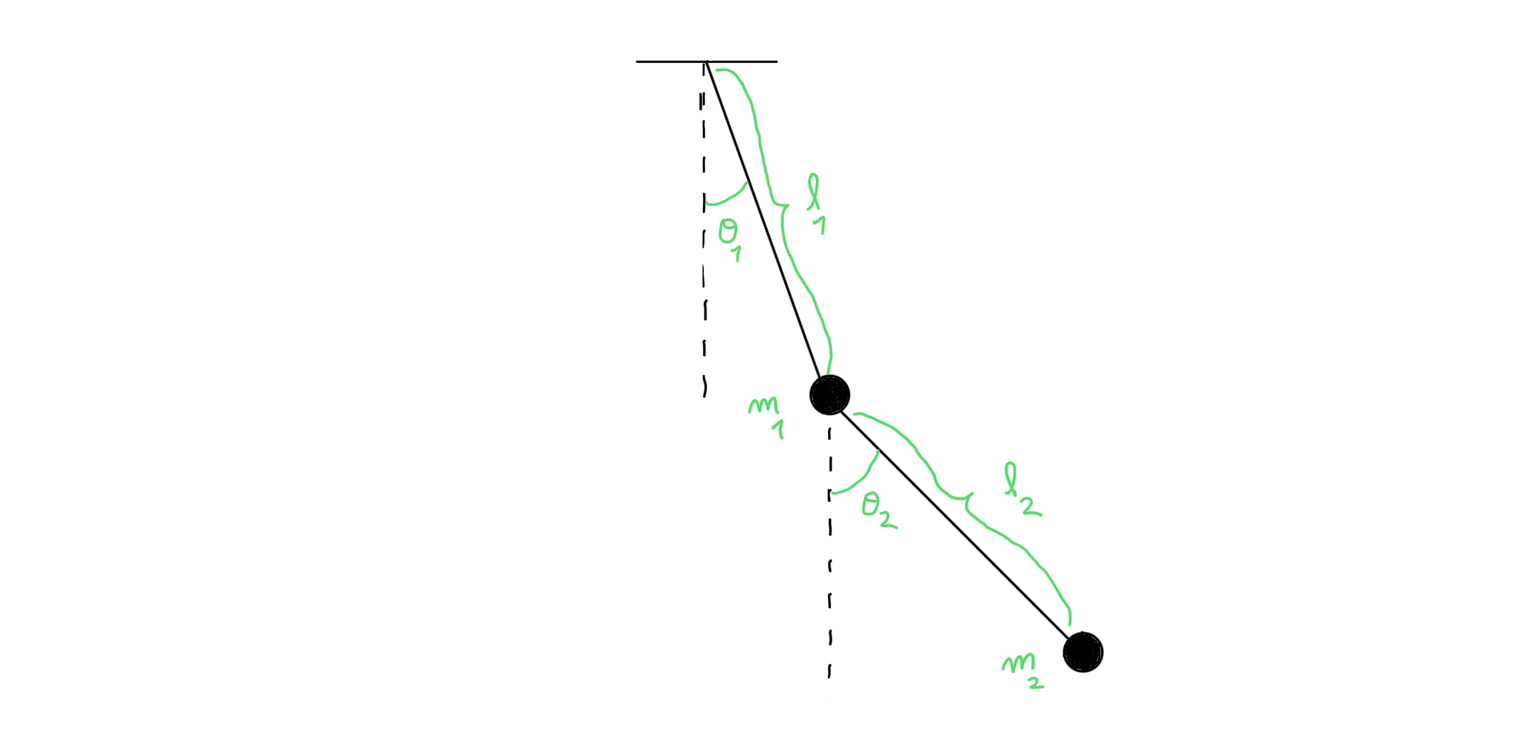
\includegraphics[scale=0.2]{schema_double_pendule.png}
  \caption{Double pendule}
  \label{fig:double pendule}
\end{figure}
\\
\subsection{Mise en équation}
On remarque alors que déterminer les angles $\theta_1$ et $\theta_2$ à tout instant permettra de connaître le mouvement du double pendule et donc de résoudre ce problème.\\
En appliquant les équations de Lagrange, on obtient les équations du mouvement que vérifient $\theta_1$ et $\theta_2$ :
$$
\left\{
\begin{array}{lcl}
    (m_1 + m_2)l_1\theta_1''(t) + m_2l_2\theta_2''(t)\cos(\theta_1(t) - \theta_2(t)) + m_2l_2\theta_2'(t)^2\sin(\theta_1(t) - \theta_2(t)) + (m_1 + m_2)g\sin(\theta_1(t)) = 0\\
    l_1\theta_1''(t)\cos(\theta_1(t) - \theta_2(t)) + l_2\theta_2''(t) - l_1\theta_1'(t)^2\sin(\theta_1(t) - \theta_2(t)) + g\sin(\theta_2(t)) = 0, \forall t \geq 0
\end{array}
\right.
$$
Posons
$$
X(t) := \begin{pmatrix}
    \theta_1(t)\\
    \theta_2(t)\\
    \theta_1'(t)\\
    \theta_2'(t)
\end{pmatrix}, \forall t \geq 0
$$
Posons ensuite :
$$
A(X(t)) := \begin{bmatrix}
    (m_1 + m_2)l_1 & m_2l_2\cos(\theta_1(t) - \theta_2(t))\\
    l_1\cos(\theta_1(t) - \theta_2(t)) & l_2
\end{bmatrix}, \forall t \geq 0
$$
et
$$
b(X(t)) := \begin{pmatrix}
    -m_2l_2\theta_2'(t)^2\sin(\theta_1(t) - \theta_2(t)) - (m_1 + m_2)g\sin(\theta_1(t))\\
    l_1\theta_1'(t)^2\sin(\theta_1(t) - \theta_2(t)) - g\sin(\theta_2(t))
\end{pmatrix}, \forall t \geq 0
$$
Alors le système d'équations devient :
$$
A(X(t))\begin{pmatrix}
    \theta_1''(t)\\
    \theta_2''(t)
\end{pmatrix} - b(X(t)) = 0, \forall t \geq 0
$$
autrement dit :
$$
A(X(t))\begin{pmatrix}
    \theta_1''(t)\\
    \theta_2''(t)
\end{pmatrix} = b(X(t)), \forall t \geq 0
$$
Remarquons que, pour tout $t \geq 0$, $A(X(t))$ est inversible. En effet, pour tout $t \geq 0$ :
$$
\Delta(X(t)) := \det A(X(t)) = l_1l_2(m_1 + m_2(1 - \cos^2(\theta_1(t) - \theta_2(t)))) \geq l_1l_2m_1 > 0
$$
En particulier, pour tout $t \geq 0$, $\Delta(X(t)) \neq 0$.\\
Par conséquent :
$$
\begin{pmatrix}
    \theta_1''(t)\\
    \theta_2''(t)
\end{pmatrix} = A^{-1}(X(t))b(X(t)), \forall t \geq 0
$$
avec $A^{-1}(X(t)) = \frac{1}{\Delta(X(t))}\begin{bmatrix}
    l_2 & -m_2l_2\cos(\theta_1(t) - \theta_2(t))\\
    -l_1\cos(\theta_1(t) - \theta_2(t)) & (m_1 + m_2)l_1
\end{bmatrix}, \forall t \geq 0$
\subsection{Etude qualitative}
Pour étudier ce système d'EDO, on commence par écrire l'équation sous la forme d'un problème de Cauchy.\\
On a : $X'(t)=\begin{pmatrix}
    \theta_1'(t)\\
    \theta_2'(t)\\
    \theta_1''(t)\\
    \theta_2''(t)
\end{pmatrix}$ pour tout t$\geq$0\\
Or d'après les équations de mouvement :
\\$X'(t) = \begin{pmatrix}
    \theta_1'(t)\\
    \theta_2'(t)\\
    A^{-1}(X(t))b(X(t))
\end{pmatrix}$\\
On note donc $f$ la fonction définie par : \begin{cases}
    $$
    \mathbb{R} \times \mathbb{R}^4 \longrightarrow \mathbb{R}^4\\
    (t,y=(y_1,y_2,y_3,y_4)) \longmapsto \begin{pmatrix}
    y_3\\
    y_4\\
    A^{-1}(y)b(y)
    \end{pmatrix}
    $$
\end{cases}\\
On a alors : $X'(t) = f(t,X(t))$, pour tout $t \geq 0$\\
L'équation devient donc : \begin{cases}
    $$
    X'(t) = f(t,X(t)), & \forall t \geq 0\\
    X(0) = \begin{pmatrix}
    \theta_{1,0}\\
    \theta_{2,0}\\
        0\\
        0
    \end{pmatrix} := X_0
    $$
\end{cases}
\subsubsection{Existence d'une solution maximale}
Par manque de temps et de place dans le rapport, ce paragraphe est laissé au lecteur. Je vous laisse montrer que l'équation différentielle admet une unique solution, qui est donc $X = \begin{pmatrix}
    \theta_1 \\
    \theta_2 \\
    \theta_1' \\
    \theta_2'
\end{pmatrix}$ (appliquer le théorème de Cauchy-Lipschitz).
\subsection{Etude numérique}
Pour l'étude numérique, c'est exactement la même chose que pour le pendule simple et le pendule couplé. Je vous laisse regarder les fichiers par vous-même et les exécuter afin de réaliser une simulation numérique du double pendule. Si vous y arrivez, c'est que vous avez bien compris le raisonnement général.
\section{Conclusion}
Durant ce projet, nous avons exploré trois problèmes physiques liés aux pendules en simulant numériquement leur oscillation à partir des \gls{edo} que vérifient les angles. Nous voyons donc l'importance de l'étude des \gls{edo} et de leur approximation numérique dans l'étude des problèmes en physique. Néanmoins, remarquons que ces trois problèmes sont des problèmes uniquement temporels. En effet, les grandeurs (ici les angles) qu'on cherche a déterminer (ou plus exactement à approcher numériquement) ne dépendent que du temps, c'est-à-dire que d'une variable réelle. Cette branche des mathématiques a donc des limites. Par exemple, elle ne s'applique pas quand il y a des perturbations de proche en proche (propagation des ondes, diffusion de la chaleur, ...), c'est-à-dire il y a en plus d'une évolution temporelle une évolution spatiale, et donc la grandeur qu'on cherche à déterminer (cf hauteur d'une vague, température dans une pièce, ...) dépend à présent de plusieurs variables réelles (temps et position dans l'espace). Dans ce type de problèmes, il y aura donc des dérivées partielles qui apparaissent dans les équations (cf représentation d'une vague). Mais comment fait-on me diriez-vous ?\\
A suivre en MACS 2 durant le cours sur les Equations aux Dérivées Partielles (EDP linéaires et Différences Finies)...\\

\begin{tcolorbox}
\begin{rem}
Durant le projet, nous avons majoritairement utilisé le raisonnement par l'absurde. Cela provient du fait que nous excluons les différents cas possibles pour garder un seul candidat. C'est comme si l'\gls{edo} "forçait" la fonction à prendre telle ou telle direction, l'empêchant de prendre les autres directions.
\end{rem}
\end{tcolorbox}

N.B. Pour l'étude qualitative des \gls{edo} pour le problème du pendule couplé et du double pendule, nous aurions pu aller plus loin à l'instar du pendule simple, mais par manque de temps et de place, nous ne l'avons pas fait. On voit donc une amélioration possible dans ce projet...
\newpage
\section{Annexe}
\subsection{Asymptote horizontale en l'infini}
\begin{tcolorbox}[colback=green!5!white, colframe=green!50!black]
\begin{prop}
Soit $f : \mathbb{R} \longrightarrow \mathbb{R}$ une fonction .\\
Si $f$ admet une limite finie en $+\infty$, est dérivable et $f'$ admet une limite finie en $+\infty$, alors
$$
\lim_{x\to+\infty} f'(x) = 0
$$
\end{prop}
\end{tcolorbox}
\begin{figure}
  \centering
  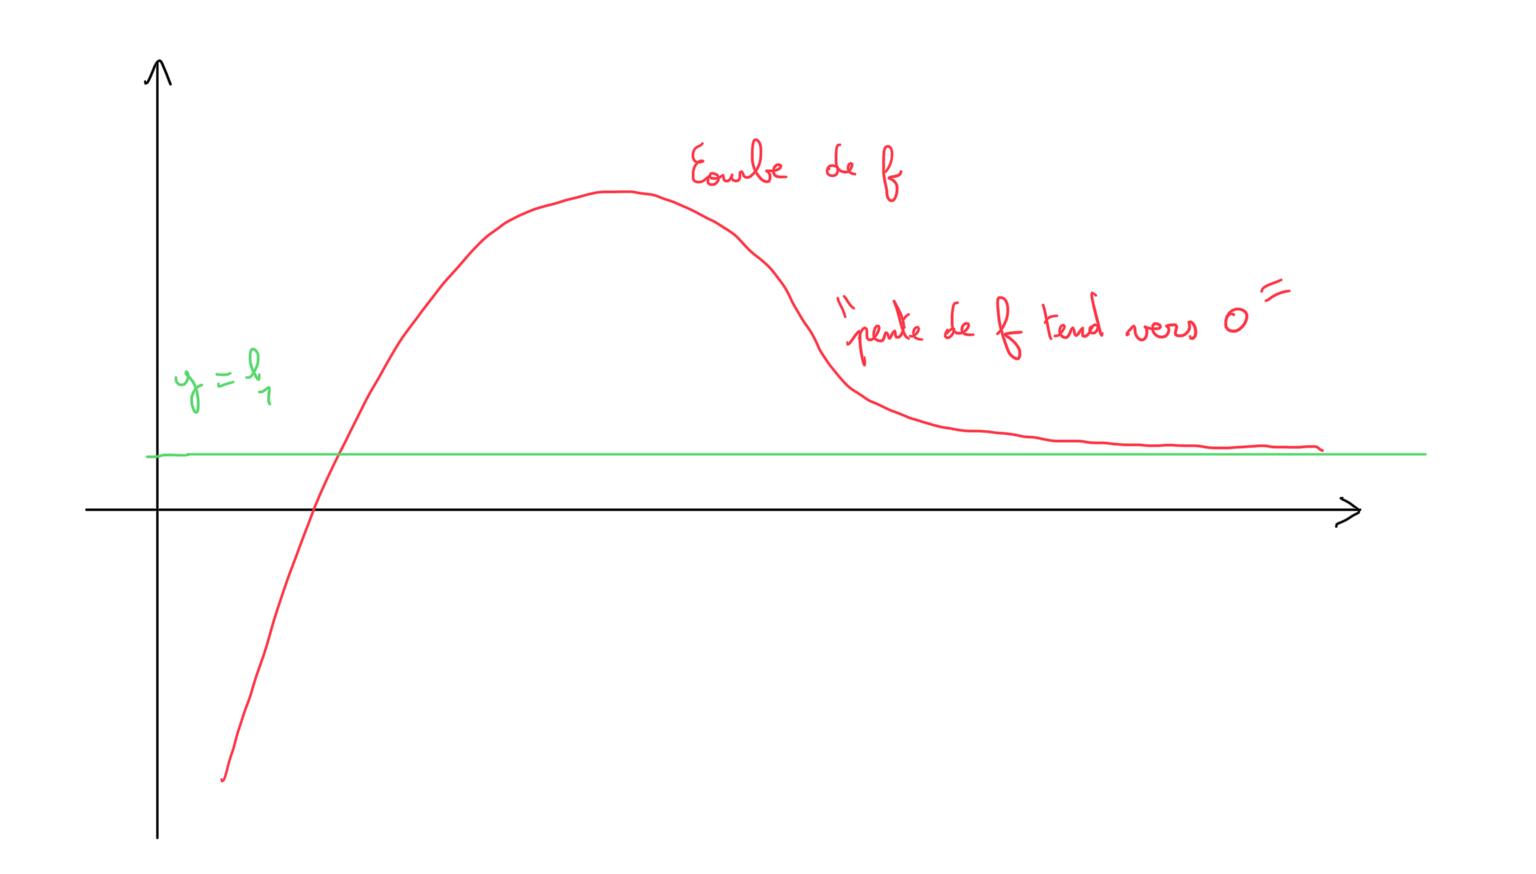
\includegraphics[scale=0.2]{illustration_asymptote.png}
  \caption{Illustration de la proposition 4}
  \label{fig:illustration proposition}
\end{figure}
\textbf{\textit{Preuve}} : Notons $l_1$ la limite de $f$ en $+\infty$ et $l_2$ la limite de $f'$ en $+\infty$. Montrons que $l_2 = 0$.\\
Puisque $\lim_{x\to+\infty} f(x) = l_1$, on a par définition de la limite :
$$
\forall \epsilon > 0, \exists A \in \mathbb{R}, \forall x \geq A, |f(x) - l_1| \leq \epsilon
$$
Par conséquent, pour tout $n > 0$, il existe $A_n \in \mathbb{R}$ tel que pour tout $x \geq A_n$, $|f(x) - l_1| \leq \frac{1}{2n}$.\\
On va à présent construire deux suites par récurrence.\\
On considère d'abord la suite réelle $(x_{1, n})_{n \in \mathbb{N}^*}$ définie par :
$$
\left\{
  \begin{array}{lcl}
    x_{1, 1} = A_1 \\
    x_{1, n + 1} = max(A_{n + 1}, x_{1, n} + 1), & \forall n \in \mathbb{N}^* \\
  \end{array}
\right.
$$
On considère ensuite la suite réelle $(x_{2, n})_{n \in \mathbb{N}^*}$ définie par $x_{2, n} = x_{1, n} + 1$, pour tout $n \in \mathbb{N}^*$ de sorte que $x_{2, n} - x_{1, n} = 1$, pour tout $n \in \mathbb{N}^*$. Soit $n \in \mathbb{N}^*$. Alors :
$$
|f(x_{2, n}) - f(x_{1, n})| = |f(x_{2, n}) - l_1 + l_1 - f(x_{1, n})| \leq |f(x_{2, n}) - l_1| + |f(x_{1, n}) - l_1| \leq \frac{1}{2n} + \frac{1}{2n} = \frac{1}{n}
$$
Or, puisque $f$ est continue sur $[x_{1, n}, x_{2, n}]$ et dérivable sur $]x_{1, n}, x_{2, n}[$, par le théorème des accroissements finis, il existe $x_n \in ]x_{1, n}, x_{2, n}[$ tel que :
$$
f(x_{2, n}) - f(x_{1, n}) = f'(x_n)(x_{2, n} - x_{1, n}) = f'(x_n)
$$
et donc :
$$
|f'(x_n)| = |f(x_{2, n}) - f(x_{1, n})| \leq \frac{1}{n}
$$
Or, $\lim_{n\to+\infty} \frac{1}{n} = 0$. Donc par le théorème de l'encadrement :
$$
\lim_{n\to+\infty} f'(x_n) = 0
$$
De plus, puisque pour tout $n \in \mathbb{N}^*, x_{1, n + 1} - x_{1, n} \geq 1$ (par construction de la suite), alors :
$$
\lim_{n\to+\infty} x_{1, n} = +\infty
$$
et donc, par le théorème de comparaison :
$$
\lim_{n\to+\infty} x_n = +\infty
$$
On a ainsi construit une suite $(x_n)_{n \in \mathbb{N}^*}$ tel que :
$$
\left\{
  \begin{array}{lcl}
    \lim_{n\to+\infty} x_n = +\infty \\
    \lim_{n\to+\infty} f'(x_n) = 0 \\
  \end{array}
\right.
$$
Or :
$$
\left\{
  \begin{array}{lcl}
    \lim_{n\to+\infty} x_n = +\infty \\
    \lim_{x\to+\infty} f'(x) = l_2 \\
  \end{array}
\right.
$$
et donc :
$$
\lim_{n\to+\infty} f'(x_n) = l_2
$$
Pour résumer, on vient de montrer que :
$$
\left\{
  \begin{array}{lcl}
    \lim_{n\to+\infty} f'(x_n) = 0 \\
    \lim_{n\to+\infty} f'(x_n) = l_2 \\
  \end{array}
\right.
$$
Finalement, par unicité de la limite, on en déduit que $l_2 = 0$, ce qui achève la démonstration.
\subsection{Mise en équation du pendule couplé}
Nous allons montrer dans ce paragraphe comment obtenir le système d'équations du pendule couplé.
Vous trouverez ci-dessous le schéma du pendule couplé.\\
Commençons par étudier le premier pendule :
\begin{itemize}[label=\textbullet]
    \item Bilan des forces
    \begin{itemize}[label=\textbullet]
        \item $\vec{P_1} = m_1\vec{g}$, où $\vec{g} = g\vec{u_x} = g(\cos(\theta_1)\vec{u_{r_1}} - \sin(\theta_1)\vec{u_{\theta_1}})$\\
        $\vec{P_1} = m_1g\cos(\theta_1)\vec{u_{r_1}} - m_1g\sin(\theta_1)\vec{u_{\theta_1}}$
        \item $\vec{T_1} = -T_1\vec{u_{r_1}}$
        \item $\vec{F_{R_1}} = ka(\sin(\theta_2) - \sin(\theta_1))\vec{u_y} = ka(\sin(\theta_2) - \sin(\theta_1))\sin(\theta_1)\vec{u_{r_1}} + ka(\sin(\theta_2) - \sin(\theta_1))\cos(\theta_1)\vec{u_{\theta_1}}$
    \end{itemize}
    \item Calcul du moment des forces
    \begin{itemize}[label=\textbullet]
        \item $\vec{M_{O_1}}(\vec{P_1}) = l\vec{u_{r_1}} \wedge \vec{P_1} = -lm_1g\sin(\theta_1)\vec{u_z}$
        \item $\vec{M_{O_1}}(\vec{T_1}) = \vec{0}$
        \item $\vec{M_{O_1}}(\vec{F_{R_1}}) = a\vec{u_{r_1}} \wedge \vec{F_{R_1}} = a^2k(\sin(\theta_2) - \sin(\theta_1))\cos(\theta_1)\vec{u_z}$
    \end{itemize}
    \item Calcul du moment cinétique
    \begin{itemize}[label=\textbullet]
        \item $\vec{L_{O_1}}(M_1) = l\vec{u_{r_1}} \wedge m_1l\theta_1'\vec{u_{\theta_1}} = m_1l^2\theta_1'\vec{u_z}$
    \end{itemize}
    \item Le théorème du moment cinétique nous affirme que :
    $$
    \vec{L_{O_1}}'(M_1) = \vec{M_{O_1}}(\vec{P_1}) + \vec{M_{O_1}}(\vec{T_1}) + \vec{M_{O_1}}(\vec{F_{R_1}})
    $$
    c'est-à-dire :
    $$
    m_1l^2\theta_1''\vec{u_z} = -lm_1g\sin(\theta_1)\vec{u_z} + a^2k(\sin(\theta_2) - \sin(\theta_1))\cos(\theta_1)\vec{u_z}
    $$
    ou encore :
    $$
    m_1l^2\theta_1'' + lm_1g\sin(\theta_1) - a^2k(\sin(\theta_2) - \sin(\theta_1))\cos(\theta_1) = 0
    $$
\end{itemize}
Le raisonnement pour le deuxième pendule est analogue, à la différence près que $\vec{F_{R_2}} = -\vec{F_{R_1}}$. On obtient ainsi :
$$
m_2l^2\theta_2'' + lm_2g\sin(\theta_2) + a^2k(\sin(\theta_2) - \sin(\theta_1))\cos(\theta_2) = 0
$$
Ainsi, on aboutit comme convenu au système d'équations suivant :
$$
\left\{
\begin{array}{lcl}
    m_1l^2\theta_1''(t) + m_1gl\sin(\theta_1(t)) - a^2k(\sin(\theta_2(t)) - \sin(\theta_1(t)))\cos(\theta_1(t)) = 0, & \forall t \geq 0 \\
    m_2l^2\theta_2''(t) + m_2gl\sin(\theta_2(t)) + a^2k(\sin(\theta_2(t)) - \sin(\theta_1(t)))\cos(\theta_2(t)) = 0, & \forall t \geq 0 \\
\end{array}
\right.
$$
Je tiens à préciser que j'ai supposé les forces de rappel du ressort horizontales pour faciliter la mise en équation (ce qui est faux mais c'est une "bonne" approximation pour des angles "petits").
\begin{figure}
  \centering
  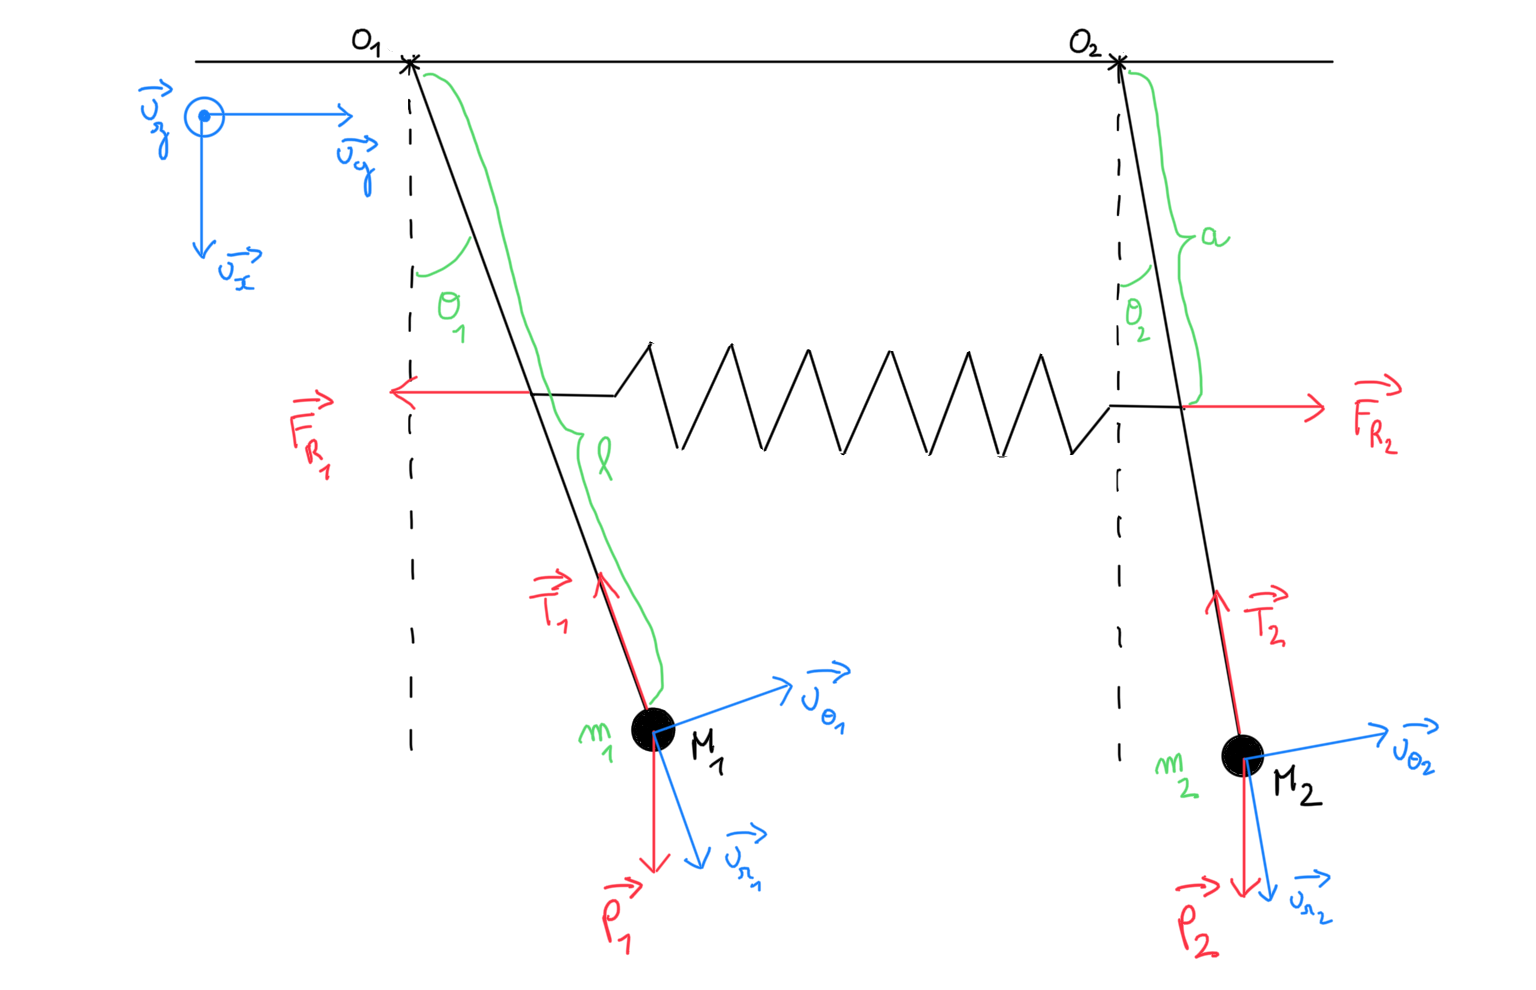
\includegraphics[scale=0.2]{schema_pendule_couple.png}
  \caption{Pendule couplé}
  \label{fig:pendule couplé}
\end{figure}

\newpage

\begin{thebibliography}{9}
\bibitem{vauchelet}
Nicolas Vauchelet (2023) : \emph{Cours sur les \gls{edo} (MACS 1)}

\bibitem{mans}
Le Mans Université : \emph{page internet}, \url{http://subaru.univ-lemans.fr/AccesLibre/UM/Pedago/physique/02/meca/coupressort.html}

\bibitem{wikipedia1}
Wikipédia : \emph{page internet}, \url{https://fr.wikipedia.org/wiki/Pendule_double}

\bibitem{wikipedia2}
Wikipédia : \emph{page internet}, \url{https://fr.wikipedia.org/wiki/Th%C3%A9or%C3%A8me_du_moment_cin%C3%A9tique}
\end{thebibliography}

\end{document}
